\documentclass[thesis.tex]{subfiles}
\begin{document}
\chapter{Introduction}

\todo{%
  This chapter should introduce:
  \begin{itemize}
  \item Introduce the thesis.
  \item State the main contributions.
  \end{itemize}

  We should also ask \emph{what is the thesis of the thesis} which is a fiddly
  way of asking what are we trying to prove with this document?
}

\subsection{The Need For Policies}

With mobile devices becoming increasingly capable and holding
ever-increasing amounts of information there is a need from users and
businesses to manage how the devices behave.  Employees now bring
their mobile devices to work and use them to access company email and
documents.  In response to this companies publish mobile device
policies that describe how the devices should be used within the
company.  These policies vary in terms of formality.  A user may never
write their privacy preferences in a formal language, but they may
make decisions guided by them.  For example which apps to install and
which to avoid.  They may make decisions based on what their friends
have told them, or what a review said about the app.  They may also
use \ac{MDM} software to enforce the policies.  If a company wishes to
use an app for business purposes there may be regulation they need to
follow, such as \ac{HIPAA}.

A company looking to control the mobile devices their employees bring
to work might write a \ac{BYOD} policy.  They might also use \ac{MDM}
software to control some aspects of their devices.  The company might
write these with varying degrees of formality but often they are
written using natural language.  This adds vagueness and can lead to
confusion as to how a policy should be implemented.  By describing the
policy in a formal language we can start to express the policy more
rigorously.  We can start to make comparisons between users, and with
rules for checking the policy start to help the user to make decisions
more accurately, or measure the extent a user follows their stated
policy.  Using formal languages we can
model the policies precisely, helping clarify their meanings and make
precise comparisons between different policies.  We can tie the rules
in the \ac{BYOD} policies, for example, to the \ac{MDM} tools used to
implement them.

If a company needs to use apps which conform with a policy such as
\ac{HIPAA} they could use static analysis tools to check for some
aspects of the policy.  Perhaps the company might use
Mallodroid~\cite{fahl_why_2012} to detect when data is sent
unencrypted.  It is important, however, not to confuse the tools and
techniques we might use to implement parts of a policy with the end
goal of ensuring that the policy is followed.  A formal language that
lets us sever the policy from its implementation can help us
understand the policy precisely, and then show precisely how the
policy is checked.  It lets us see what rules from the policy are
checked for by which tools, and identify gaps where the policy is not
being checked sufficiently.

A key aspect of the mobile ecosystem is delegation.  The user of a
mobile device (typically) first logs on to a Google or Apple account
before using the device, which retrieves all their data.  Even in an
app rather than store all the data locally the app may prompt the user
to log in and delegate to a third-party (such as Google or Facebook)
to manage the account ID.

Users may install apps manually themselves, but they might use one or
more app stores to provide them with apps.  They trust these app
stores to provide them with \emph{good and safe} apps, and delegate
the checking of them to the store.  Whereas a user might once have
done the check themselves (or at least delegated to an \ac{AV} package
on their computer) now the responsibility is handed to the stores.
Furthermore all software comes signed either by the developer who
created it (in the case of Google's Play Store), the store that sold
it (in the case of Amazon's app store) or both (Apple's App Store).  A
store may delegate to a third-party app vetting service to determine
what apps are safe (Yandex and Aptoide stores), or use their own
in-house teams.

On Android there is a requirement that whenever
an app is updated the update's signature must be from the same key as
the app it is updating.  This means that there is a delegation from
the OS to the developer to say what is a valid update, but also a
trust relationship from the user to the developer (or store) to
provide updates at all, as no-one else will be able to patch the
software.

Users recommend each other apps.  Some may consider what apps they
want to use on their phone and come up with internalized policies that
describe how they want to use them, and may trust reviews to give them
an idea of an app's quality, and the phone itself to tell them what
functionality the app has through its permissions.

They allow their employers to say how they should their devices, who
may in turn delegate to IT departments, to write rules, which may
delegate back to the users to state what rules they're willing to
follow.

These trust relationships and delegations permeate the entire mobile
ecosystem.  They represent an important aspect of the ecosystem that a
policy language should catch in order to adequately describe the
relationships and policies within it.

One approach to designing a policy language is to base it on a logic
of authorization.  These authorization logics describe rules for
deciding when an action is permitted, and reasoning about why that
action was allowed.  A common use case for these logics is building
access control systems: users are allowed to read a file if they have
the appropriate permissions.  In applying logics of authorization to
policy language the policy language describes who can access what, but
the authorization logic gives a formal description of how we make that
decision.

We need an authorization language for mobile ecosystems.


\subsection{History of Mobile Devices}

Some of the earliest mobile devices were the \acp{PDA} devices of the
early 90s.  The earliest devices, such as Apple's Newton, were
portable miniature computers designed to store personal information,
calendars and notes.  Developers could even program additional apps
for them (in the case of the Newton using Apple's Dylan language).  At
the time mobile phones were just portable telephones, but starting
with the IBM Simon in 1994 these devices started to have some of the
functionality of the \ac{PDA}, becoming what would later be called a
\emph{smart phone}.  The big advantage of these early smart phones
over the \ac{PDA} was they had a telephone connection.  The earliest
devices allowed their users to access email and fax, as well as
managing personal information.  The early smart phones were somewhat
underpowered compared to the \ac{PDA} devices so both continued to
develop alongside one another, and started to become more affordable.

In 1998 the Symbian OS was released.  Developed by Psion (who made
\acp{PDA}), and Motorola, Ericsson and Nokia (all phone
manufacturers).  By the early 2000s it would start to become the
dominant smart phone OS.  These devices could install apps, written in
C++ or Java (if the phone supported JME). They had cameras, could play
music. They even had early malware which would illicitly send texts to
premium rate numbers.  They were the forebears of the \emph{modern}
smart phone.
They were also starting to become affordable, with the lowest end
models starting to being affordable by children and
teenagers\footnote{If you saved up for what seemed like
  forever$\ldots$}.  Devices like Nokia's N-Gage were marketed directly
towards these younger users and featured games users could buy for
their devices.

In the mid-2000s we first start to see the mobile
ecosystem proper.  We have users with different devices, downloading
apps from different sources (some pirated).  These devices
contained personal information of the \acp{PDA}, but also photographs
and music.  Users could browse the web, and send each other pictures.
With increasing amounts of personal information malware authors
started to take note.  In a blog post from 2006 for Symantec, Chien
noted~\cite{eric_chien_spyware_2006}:

\begin{quote}
  ``While threats exist and are actively spreading, we are probably
  still years away from the situation we have with the Microsoft Windows
  [$\cdots$] We have already seen spyware applications for mobile devices
  (e.g. Spyware.Flexispy) that can monitor activities on the mobile
  device and then send them to a remote server. [$\cdots$] Just as
  worrying is the fact that the adware market is just beginning to take
  notice of mobile devices. Already some Bluetooth advertising schemes
  have been tested, where a bus stop is outfitted with a device that
  just spams out messages via Bluetooth.

  [$\cdots$]
  
  So, while worms and Trojans already exist for the mobile
  platforms, spyware and adware applications are just now gaining a
  foothold in the mobile device space. Spyware and adware pose a
  potentially large security issue in the near future, as the companies
  that produce such applications are less affected by the natural
  limiting factors.''
\end{quote}

In 2008 Apple released the first iPhone, and shortly after Google
released the Android OS.  Symbian would release its final version in
2012, with Android as the dominant OS on most devices.  These
operating systems differed from past efforts, and conventional desktop
OS, in that they were far more controlled than previous systems.
Apple's devices could not run code that Apple had not signed or
install software from outside of its App Store, which Apple
controlled.  Android devices offered a similar app marketplace, but
where there seemed to be less checking of individual
apps~\cite{oberheide_dissecting_2012}. Whilst Android users could
install software from other sources, the option was hidden by default.
As well as restrictions to software, these devices were also better
protected.  Devices no longer had an all powerful \emph{root} account.
APIs were provided that restricted malicious behaviors.  One example
was stopping SMSs being sent programatically to premium rate accounts;
essentially ending a monetization technique that had been prevelent in
malware before. 

Mobile devices stored a large amount of personal data about their
users.  They contained address books, records of phone calls, and GPS
logs of where their users had been.  With iOS and Android user's
became more aware about privacy on their devices, in part because of
increased media coverage of privacy issues.  A survey in 2012 by
Chin~et~al{.} found that users were more concerned about privacy on
their mobile devices, than on their
laptops~\cite{chin_measuring_2012}. Users of a smartphone were more
likely to install an app that came recommended from a friend, was
popular or was free.  To subsidize the cost of producing free apps,
and to better understand how users used their apps, some developers
added adware and tracking libraries to their apps.  These libraries
accomplished a variety of tasks ranging from crash and error tracking,
to collecting personal data to be sold to advertisers to subsidize the
app's price~\cite{seungyeop_han_study_2012}.

This dynamic between users who were increasingly concerned about their
privacy and apps which were increasingly privacy invading, lead many
to argue that the mobile device operating systems needed better
controls for what data and permissions an app could
have~\cite{leontiadis_dont_2012}.  Many different schemes were
suggested to fix this and provide finer privacy
controls~\cite{jeon_dr._2012,beresford_mockdroid:_2011,conti_crepe:_2010,backes_appguard_2013}
(some of which will be described further in
\autoref{chap:related-work}).  In general, however, users did not
really understand the how app permissions
worked~\cite{felt_android_2012}.  By 2017 (and the present day) iOS
and Android had settled on a model where user's were asked by their
devices if an app could access certain data when it first requested it
and then the user could revoke that decision later if they wished.
Despite the present Android permissions model being \emph{ask on use},
a large number of older Android devices are still being used.  In June
2016 only 10\% of devices used the latest version of Android, with
around 5\% using a version more than five years old
(\autoref{fig:android-versions}).  In contrast 79\% of iOS devices use
the latest OS, 16\% use the previous version and only 5\% use anything
older~\cite{apple_app_2017}.  The greater fragmentation of the Android
versions has been attributed to the greater number of Android device
manufacturers each with their own update mechanisms as compared to
with iOS where Apple exclusively control and update all devices.

\begin{figure}
\centering
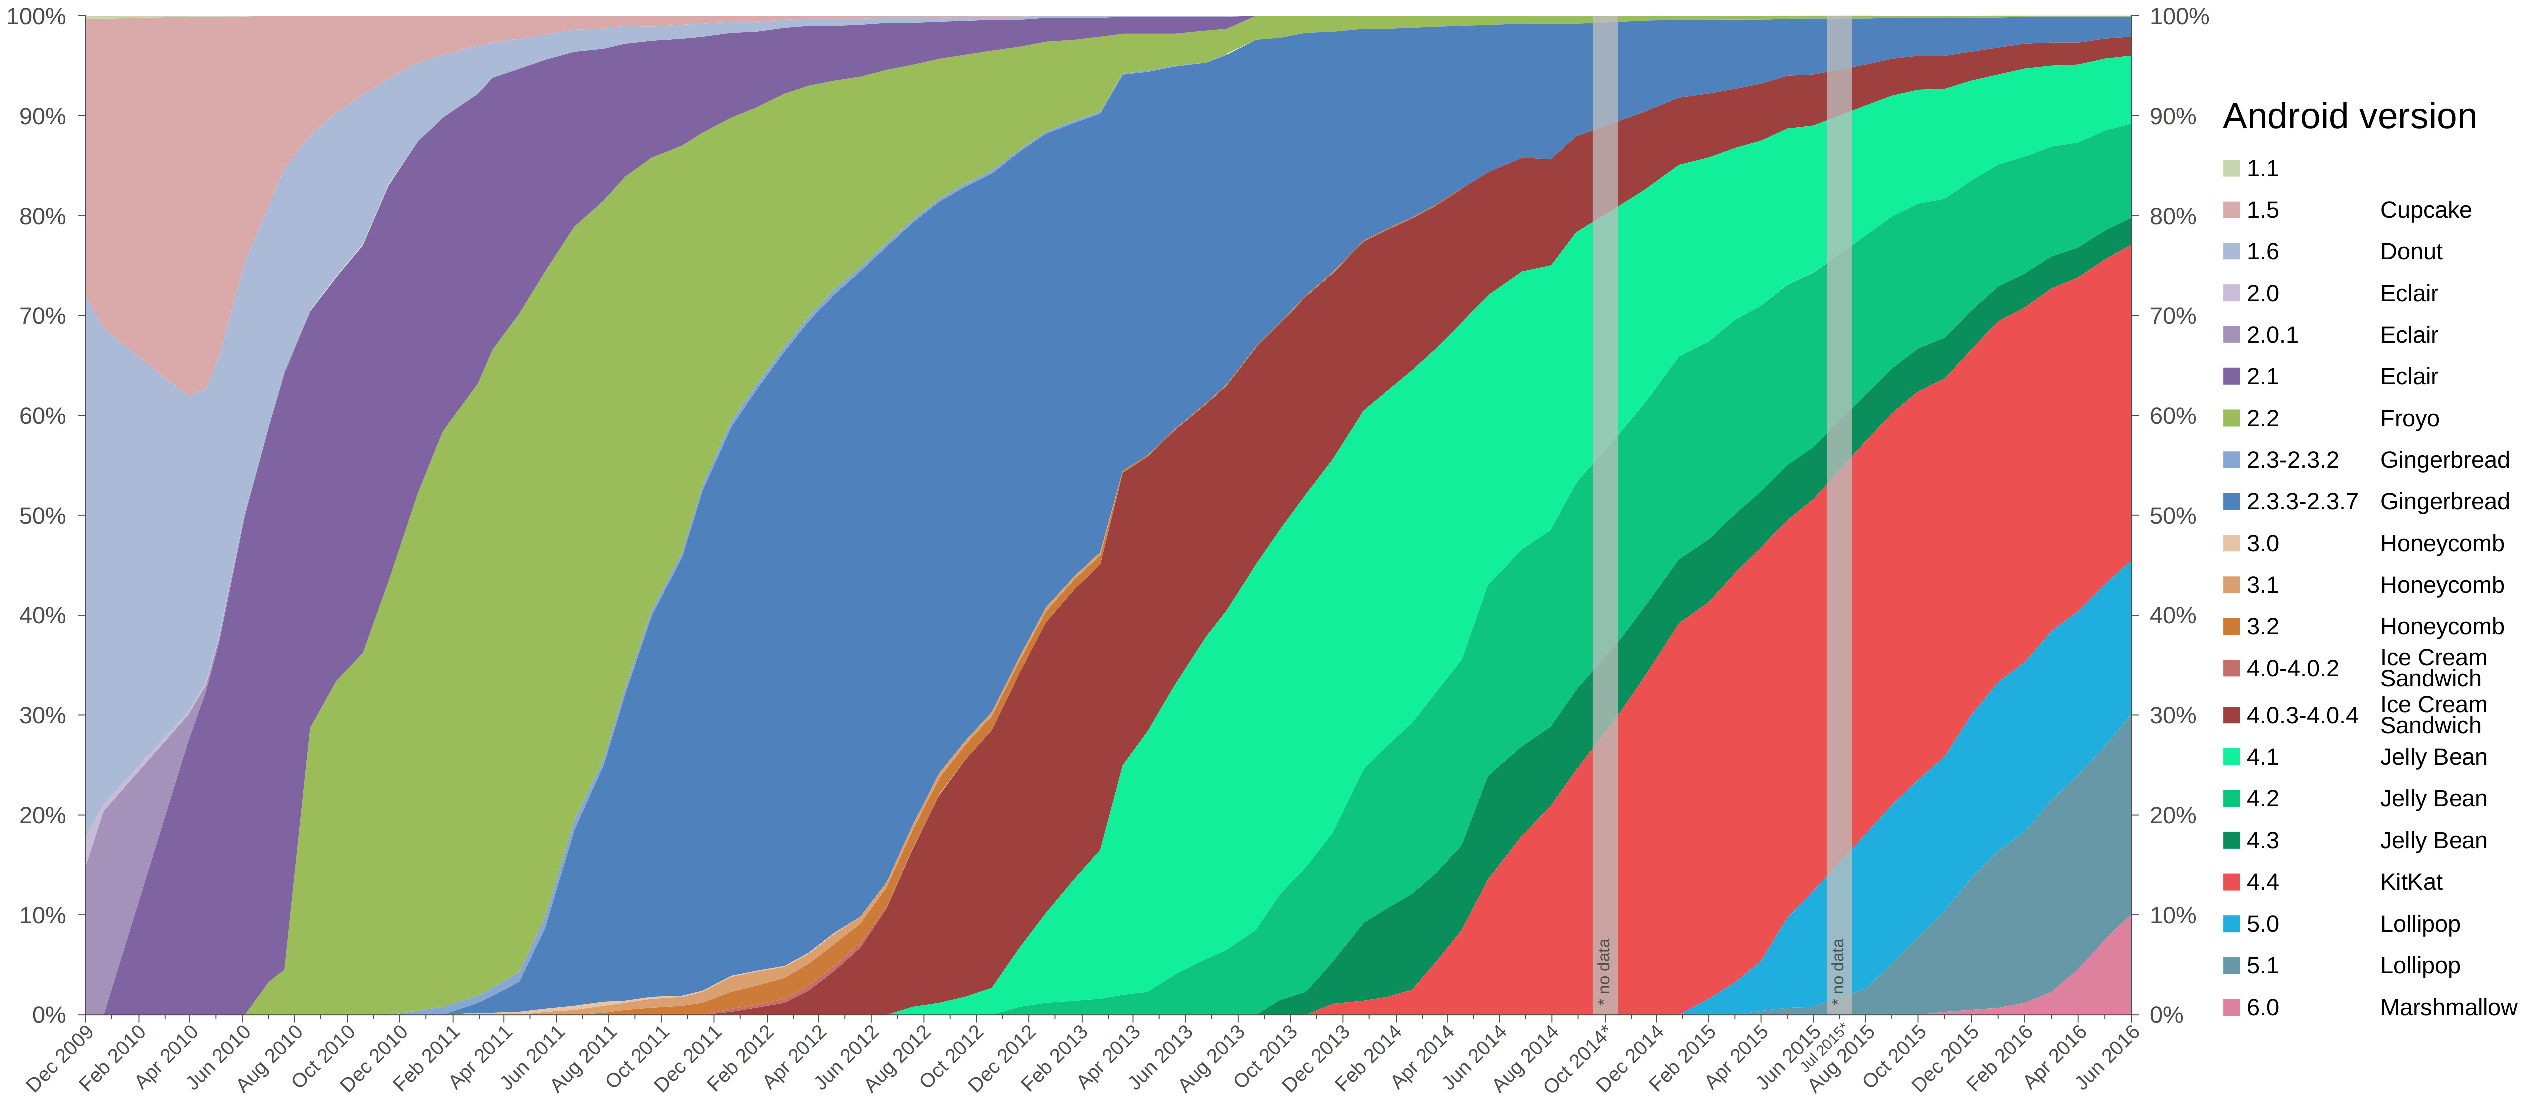
\includegraphics[width=\linewidth]{figures/android-versions.pdf}
\caption[Historical Android version's distribution.]{Historical Android
  version's distribution~\cite{erikrespo_android_2017}.}
\label{fig:android-versions}
\end{figure}

Mobile devices became more ubiquitous, and \acp{PDA} reappeared now
called \emph{tablets} or \emph{iPads}.  These devices were identical
to the smart phones, but larger and they generally did not have a
cellular data connection instead using wifi. They could not send
texts or make phone calls but a shift away from traditional SMS and
cellular phone calls to internet backed communications such as
WhatsApp, iMessage, Skype and FaceTime meant these devices were
essentially interchangeable with smart phones.

Advances in secure co-processors meant that mobile devices were even
more capable.  Banks allowed users to link their devices to their bank
accounts and use their device, or even the new \emph{smart watches} as
a debit card.  This quickly became a common and ubiquitous payment
method quickly with even street vendors, who hadn't taken cards
previously, accepting contactless payment via a mobile device.  The
separation of cryptographic operations from everyday computing with
secure co-processors and secure enclaves (such as TrustZone) lead to
significantly improved security.  Keys could be isolated from the
entire mobile OS, allowing for increased trust mechanisms.

Mobile devices gained the ability to collect increasingly personal
information.  Smart watches recorded and shared a user's pulse with
others. Mobile health apps were made to track and monitor medical
conditions. In the US, the \ac{HIPAA} required that healthcare
providers transmited medical information securely, but many apps had
basic security problems~\cite{fahl_why_2012}, and many of the
healthcare apps did not handle the medical information
securely~\cite{knorr_privacy_2015}.

\section{Publications}

The work described in this thesis builds upon work published in these publications:

\begin{itemize}
%\item \bibentry{hallett_capturing_2017}
\item 
Joseph Hallett and David Aspinall. Capturing Policies for BYOD. In \emph{IFIP Security and Privacy Conference}, 2017
%\item \bibentry{hallett_common_2017}
\item Joseph Hallett and David Aspinall. Common Concerns in BYOD Policies. \emph{In Workshop on Innovations in Mobile Privacy and Security}, April 2017
%\item \bibentry{hallett_specifying_2016}
\item Joseph Hallett and David Aspinall. Specifying BYOD Policies with Authorization Logic. \emph{In PhD Symposium at iFM'16 on Formal Methods. Reykjavik University}, June 2016
%\item \bibentry{hallett_apppal_2016}
\item Joseph Hallett and David Aspinall. AppPAL for Android. \emph{In Engineering Secure Software and Systems. Springer Verlag}, April 2016
%\item \bibentry{hallett_poster:_2015}
\item Joseph Hallett and David Aspinall. Poster: Using Authorization Logic to Capture User Policies in Mobile Ecosystems. \emph{In Symposium on Usable Privacy and Security}, 2015
%\item \bibentry{hallett_towards_2014}
\item Joseph Hallett and David Aspinall. Towards an authorization framework for app security checking. \emph{In Engineering Secure Software and Systems}, 2014
\end{itemize}


\end{document}


%%% Local Variables:
%%% mode: latex
%%% TeX-master: "../ch1"
%%% End:
